\section{Design requirements}

The Hybrid Patient Record can enhance a paper based patient record in many ways. It attempts to achieve that, through the addition of a small microcontroller that makes it possible to control LEDs, a small speaker, an RFID reader, and WiFi connectivity. \\

For instance, the record is often lost or misplaced both inside the ward or in other departments of a hospital \cite{hypr}. The HyPR device is then equipped with an ultrasound tag that broadcasts a unique value, and makes it able to be tracked down to a specific location in the hospital. A small speaker adds an identification sound for the device, and allows it be found if it is lost in a room. \\

LEDs can show a colour scheme. The colour can, for example, represent a specific nurse, a patient status or simply used in combination with sound to identify a specific device in a stack of patient journals. \\

An RFID reader reads a tag from a doctor's tablet, so they can quickly access relevant data for the associated patient. \\

WiFi capability is added in order to be able to for example, change the LED colours, or trigger the speaker. \\

Houben et al.'s proposed device shown on figure \ref{fig:old-hypr} was taken as a reference, with regards to weight, thickness and size. Although the new design retains the same purpose, the feature of having a dock for a tablet was removed, to further reduce the size. The hybrid patient record was then re-imagined to be just a thin support for a folder, with electronics on the back. \\

Working from Houben et al.'s proposed device, a new set of requirements have been established, in order to improve on the design. The following is a list of requirements pertaining to the new device:

\begin{itemize} \itemsep0em
	\item Weight: less than 500g.
	\item Thickness: less than 20mm.
	\item Size: Approximately same dimensions as A4 paper.
	\item Maintainability: easy access to the microcontroller's programming interface.
	\item Maintainability: easily change components without changing physical design.
	\item Price: each device must cost at max 1000kr.
\end{itemize}

A set of requirements pertaining to the electronic part of the device has also been decided:

\begin{itemize} \itemsep0em
	\item Rechargeable battery via standard USB cable.
	\item Battery status LEDs.
	\item Autonomy of at least 8 hours on battery, with normal use.
	\item LEDs showing colour combinations should be easily seen and understood from 10m.
	\item Hear the audio signal in a room, when device is under bed sheets.
\end{itemize}

\begin{figure}[h]
\setlength{\belowcaptionskip}{-10mm}
\begin{center}
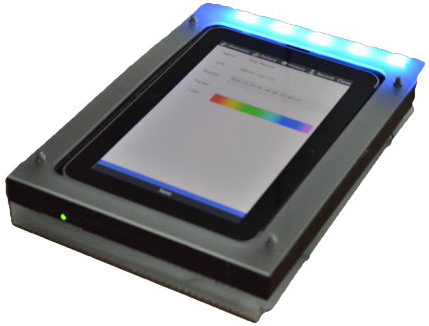
\includegraphics[scale=.5]{figures/old-hypr.jpg}
\caption{\small {\it {Houben et al.'s prototype}}} \label{fig:old-hypr}
\end{center}
\end{figure}
